\hypertarget{TestStatistic_8h}{
\section{TestStatistic.h File Reference}
\label{TestStatistic_8h}\index{TestStatistic.h@{TestStatistic.h}}
}


This graph shows which files directly or indirectly include this file:\nopagebreak
\begin{figure}[H]
\begin{center}
\leavevmode
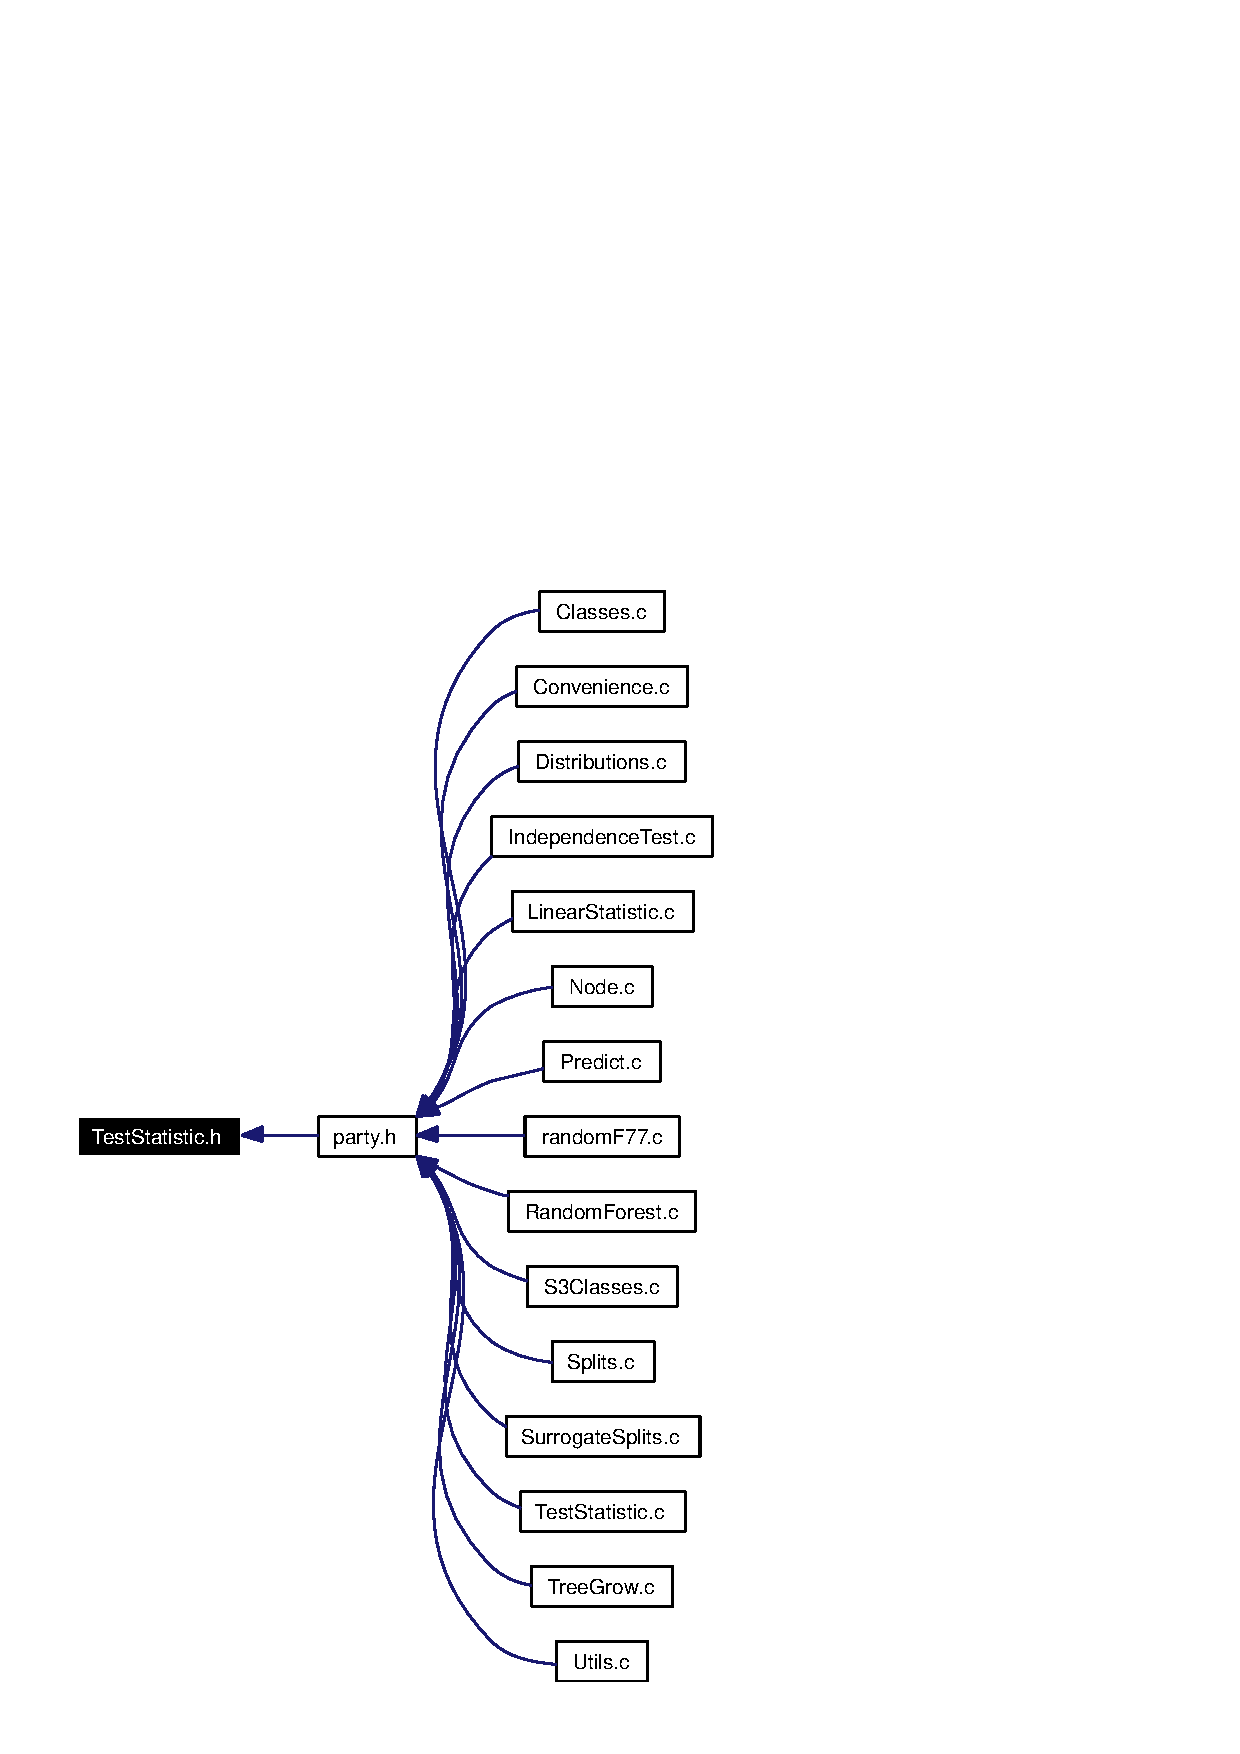
\includegraphics[width=420pt]{TestStatistic_8h__dep__incl}
\end{center}
\end{figure}
\subsection*{Functions}
\begin{CompactItemize}
\item 
void \hyperlink{TestStatistic_8h_9ecf0700a00ad5fd64601bf718f20439}{C\_\-standardize} (const double $\ast$t, const double $\ast$mu, const double $\ast$Sigma, int pq, double tol, double $\ast$ans)
\item 
double \hyperlink{TestStatistic_8h_a3a1f48e4bb3aa19d1bac85a53358638}{C\_\-maxabsTestStatistic} (const double $\ast$t, const double $\ast$mu, const double $\ast$Sigma, int pq, double tol)
\item 
double \hyperlink{TestStatistic_8h_b45eb88ec3b2cc87e8610771cdcf53c4}{C\_\-quadformTestStatistic} (const double $\ast$t, const double $\ast$mu, const double $\ast$SigmaPlus, int pq)
\end{CompactItemize}


\subsection{Function Documentation}
\hypertarget{TestStatistic_8h_a3a1f48e4bb3aa19d1bac85a53358638}{
\index{TestStatistic.h@{TestStatistic.h}!C_maxabsTestStatistic@{C\_\-maxabsTestStatistic}}
\index{C_maxabsTestStatistic@{C\_\-maxabsTestStatistic}!TestStatistic.h@{TestStatistic.h}}
\subsubsection{\setlength{\rightskip}{0pt plus 5cm}double C\_\-maxabsTestStatistic (const double $\ast$ {\em t}, const double $\ast$ {\em mu}, const double $\ast$ {\em Sigma}, int {\em pq}, double {\em tol})}}
\label{TestStatistic_8h_a3a1f48e4bb3aa19d1bac85a53358638}


Maximum absolute values of standardized statistics \begin{Desc}
\item[Parameters:]
\begin{description}
\item[{\em t}]the vector of statistics \item[{\em mu}]expectations \item[{\em Sigma}]covariance matrix \item[{\em pq}]dimension of t \item[{\em tol}]tolerance for variances \end{description}
\end{Desc}


Definition at line 66 of file TestStatistic.c.

References C\_\-absstandardize(), and C\_\-max().

Here is the call graph for this function:\nopagebreak
\begin{figure}[H]
\begin{center}
\leavevmode
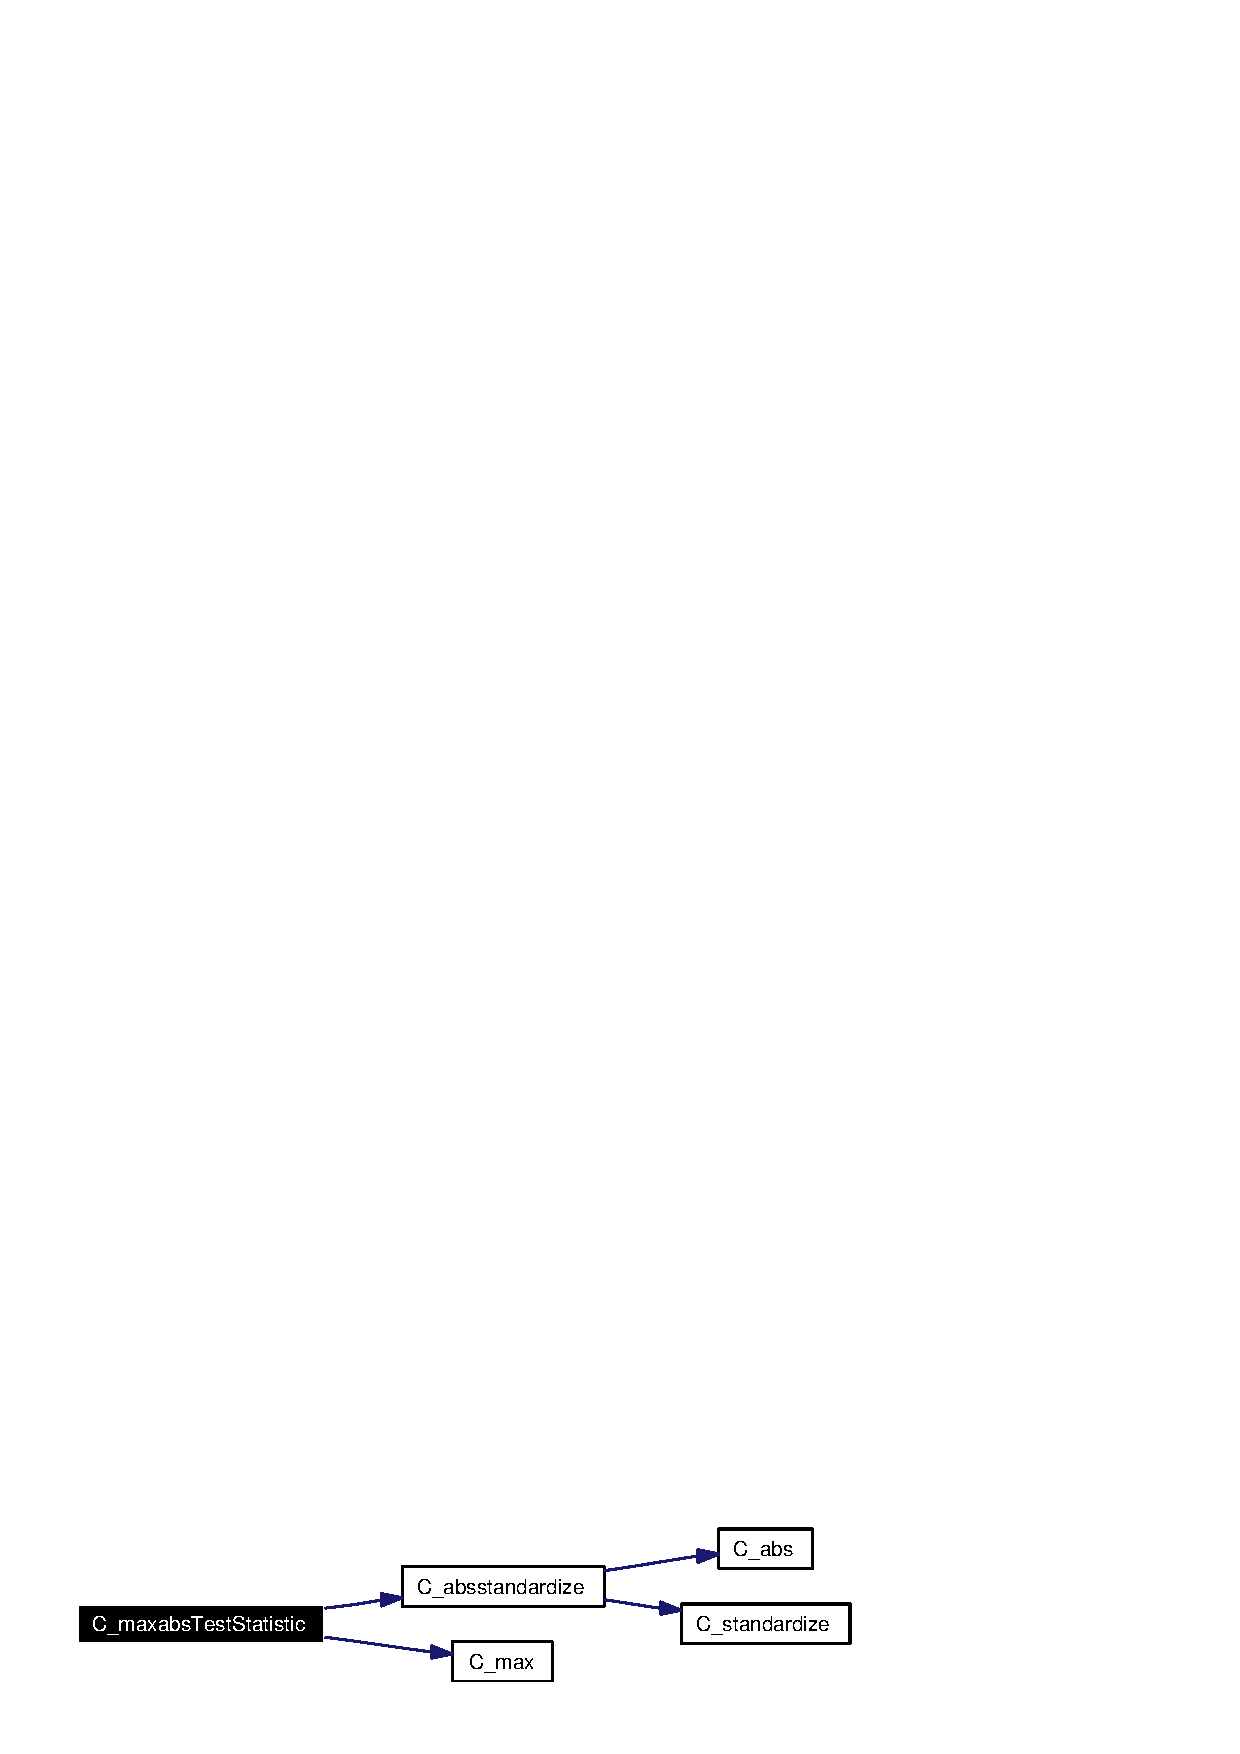
\includegraphics[width=215pt]{TestStatistic_8h_a3a1f48e4bb3aa19d1bac85a53358638_cgraph}
\end{center}
\end{figure}
\hypertarget{TestStatistic_8h_b45eb88ec3b2cc87e8610771cdcf53c4}{
\index{TestStatistic.h@{TestStatistic.h}!C_quadformTestStatistic@{C\_\-quadformTestStatistic}}
\index{C_quadformTestStatistic@{C\_\-quadformTestStatistic}!TestStatistic.h@{TestStatistic.h}}
\subsubsection{\setlength{\rightskip}{0pt plus 5cm}double C\_\-quadformTestStatistic (const double $\ast$ {\em t}, const double $\ast$ {\em mu}, const double $\ast$ {\em SigmaPlus}, int {\em pq})}}
\label{TestStatistic_8h_b45eb88ec3b2cc87e8610771cdcf53c4}


Quadratic form t(t - mu) SigmaPlus (t - mu) \par
 \begin{Desc}
\item[Parameters:]
\begin{description}
\item[{\em t}]the vector of statistics \item[{\em mu}]expectations \item[{\em SigmaPlus}]Moore-Penrose inverse \item[{\em pq}]dimension of t \end{description}
\end{Desc}


Definition at line 110 of file TestStatistic.c.\hypertarget{TestStatistic_8h_9ecf0700a00ad5fd64601bf718f20439}{
\index{TestStatistic.h@{TestStatistic.h}!C_standardize@{C\_\-standardize}}
\index{C_standardize@{C\_\-standardize}!TestStatistic.h@{TestStatistic.h}}
\subsubsection{\setlength{\rightskip}{0pt plus 5cm}void C\_\-standardize (const double $\ast$ {\em t}, const double $\ast$ {\em mu}, const double $\ast$ {\em Sigma}, int {\em pq}, double {\em tol}, double $\ast$ {\em ans})}}
\label{TestStatistic_8h_9ecf0700a00ad5fd64601bf718f20439}


Standardizes a statistic t of length pq with mean mu and covariance Sigma for variances $>$ tol \par
 \begin{Desc}
\item[Parameters:]
\begin{description}
\item[{\em t}]the vector of statistics \item[{\em mu}]expectations \item[{\em Sigma}]covariance matrix \item[{\em pq}]dimension of t \item[{\em tol}]tolerance for variances \item[{\em ans}]return value; a pointer to a REALSXP-vector of length pq \end{description}
\end{Desc}


Definition at line 23 of file TestStatistic.c.